\documentclass[a4paper,12pt]{article}
\usepackage{amsmath}
\usepackage{icomma}
\usepackage[utf8]{inputenc}
\usepackage[T1]{fontenc}
\usepackage{polski}
\usepackage[polish]{babel}
\usepackage{hyperref}
\usepackage{float}
\usepackage{graphicx}
\usepackage{subcaption}
% makra automatycznie wygenerowane z projektu za pomocą generate-macros
\newcommand{\medianfilterradius}{0,002}
\newcommand{\darkredradius}{0,3}
\newcommand{\lightredradius}{0,7}
\newcommand{\darkredthreshold}{0,2}
\newcommand{\darkblueradius}{0,3}
\newcommand{\lightblueradius}{0,9}
\newcommand{\darkbluethreshold}{0,2}
\newcommand{\openingdepth}{0,003}
\newcommand{\bestobjectscomparisondepth}{5}
\newcommand{\invarianttable}{
\begin{tabular}{l | c c c c c c c c }
Obiekt & M4 & M7 & M8 & M9 \\
\hline
Strzałka & 0.00079014 & 0.000100286 & 0 & -4.03119e-05 \\
Wagi & 1.1 & 1.2 & 0 & 0.4 \\
\hline
Litera W & 0 & -1.54905e-05 & 0 & -1.10516e-05 \\
Wagi & 0 & 1.5 & 0 & 1.5 \\
\hline
Litera K & 0.000242899 & 0 & -3.99919e-05 & -3.10566e-06 \\
Wagi & 0.8 & 0 & 0.8 & 1 \\
\hline
Litera D & 0 & 0 & -5.13758e-05 & -5.55874e-06 \\
Wagi & 0 & 0 & 1 & 0.6 \\
\hline
\end{tabular}}

\begin{document}
	\title{Warkod --- Wykrywanie loga Warszawskich Kolei Dojazdowych na zdjęciach}
	\author{Radosław Świątkiewicz}
	\date{\today}
	\maketitle
	\tableofcontents
	
	\section{Opis}
		\subsection{Stosowanie}
			Logo Warszawkich Kolei Dojazdowych ma kształt dwóch strzałek z literami pomiędzy.
			\begin{figure}
				\centering
				
\includegraphics[width=0.3\linewidth]{logo.jpg}
				\caption{Logo Warszawskich Kolei Dojazdowych}
			\end{figure}
	
		\subsection{Wymagania}
			Program jest napisany w C++ w standardzie \texttt{c++11}.
			Do pracy używa biblioteki OpenCV, testowane pod wersją \texttt{4.0.1}, ale używa jedynie podstawowych funkcji do wczytywania i zapisywania plików, które to się nie zmieniły od wcześniejszych wersji.
			Kompilacja jest możliwa za pomocą CMake.
			
		\subsection{Uruchomienie}
			Warkod jest uruchamiany z konsoli i przyjmuje dwa lub trzy argumenty.
			\begin{description}
				\item[Nazwa pliku wejściowego] to plik o dowolnym formacie, czytanym przez OpenCV.
				\item[Nazwa pliku wyjściowego] jest miejscem, gdzie program wypisze obraz wynikowy, będzie to obraz wejściowy z zaznaczonym środkiem znalezionego loga WKD.
				\item[\textsl{Opcjonalny} katalog pomocniczy] do którego będą zapisywane pliki z parametrami znalezionych obiektów, obrazy z obiektami i wstępne dopasowania.
			\end{description}
			
			Przykładowe uruchomienie:
			\texttt{./warkod zdjęcie.jpg zaznaczone.jpg /tmp}
			
	\section{Działanie}
		Program wykonuje szereg osobnych operacji.
		Wszystkie parametry kolorów zakładają, że piksel ma zakres jasności od $0,0$ do $1,0$.
		\subsection{Filtracja}
			Obraz filtrowany jest filtrem medianowym o określonej wielkości.
			Filtr jest kwadratowy o boku \medianfilterside{} pikseli. 
			Przy krawędziach zmniejsza ilość porównywanych pikseli i wybiera medianę z mniejszej ilości.
			
			Filtracja jest zaimplementowana wielowątkowo, po jednym wątku na wiersz.
			
		\subsection{Oddzielanie kolorów}
			Zastosowana została metoda porównywania geometrycznego punktów. 
			Ponieważ piksel może być zaprezentowany jako punkt we wnętrzu sześcianu, gdzie na osiach odłożone są składowe kolory czerwony, zielony i niebieski,
			można zastosować proste porównania.
			
			Wykryć należy piksele odpowiednio czerwone i niebieskie, gdyż logo składa się z takich kolorów.
			Ponieważ materiał, na którym może być logo, bywa odbijający, warto zwiększyć zakres akceptowalności dla jaśniejszych pikseli.
			
			Ciemne kolory mogą miewać różne odcienie, zależne mocno od oświetlenia, zanieczyszczeń atmosfery, itp. Mogą więc nieprawidłowo zostać zakwalifikowane.
			W tym przypadku należy odciąć zbyt ciemne piksele płaszczyzną prostopadłą do szukanego koloru.
			
			Wynikowo otrzymujemy obcięty stożek, którego szersza podstawa leży na płaszczyźnie jasnych kolorów, a obcięta podstawa jest na płaszczyźnie obcinającej po ciemnej stronie. Stożek ma wysokość równoległą do osi szukanego koloru.
			
			Każdy stożek jest identyfikowany przez 3 parametry.
			
			\begin{center}
				\begin{tabular}{ l | c  c }
					Zmienna & Niebieski kolor & Czerwony kolor \\
					\hline
					Średnica ciemna 		& \darkblueradius{} 	& \darkredradius{} \\
					Średnica jasna			& \lightblueradius{}	& \lightredradius{} \\
					Płaszczyzna ciemna		& \darkbluethreshold{}	& \darkredthreshold{} \\
				\end{tabular}
			\end{center}
			
			Tak powstałe dwa obrazy binarne są gotowe do dalszej obróbki.
			
		\subsection{Otwieranie}
			Kilkukrotne wykonanie erozji, a następnie dylacji pozwala się pozbyć małych obiektów, głównie szumu, który został zakwalifikowany do koloru, a nie został usunięty przez filtr medianowy.
			
			Głębokość otwierania zależy od wielkości obrazu, dzięki temu można w ten sam sposób przetwarzać obrazy o dowolnych rozmiarach.
			Długość mniejszego boku jest mnożona przez \openingdepth{} i zaokrąglana do części całkowitej.
			Dla większości obrazów jest to około 3.
			
			Otwieranie znacząco przyspiesza późniejsze wykrywanie obiektów, ale jeśli jest za duże, może uszkodzić literę na obrazie.
			
			Algorytm stosuje się na obu obrazach binarnych.
			Jest zaimplementowany wielowątkowo, w identyczny sposób, jak filtr medianowy.
			
		\subsection{Znajdywanie obiektów}
			Najdroższa obliczeniowo część przetwarzania.
			Należy podzielić obiekt binarny na wiele spójnych podobiektów i obliczyć charakterystyki dla każdego z nich.
			
			Odbywa się to w pętli.
			Program tworzy nowy obraz, na którym zaznacza odwiedzone piksele.
			Za każdym razem program szuka pierwszego zapalonego piksela, idąc wierszami od lewego-górnego rogu.[]
			Po znalezieniu takiego, zaczyna rozlewać, zapamiętuje znaleziony piksel w kolejce i przechodzi do głównej pętli rozlewania.
			\begin{enumerate}
				\item Pobranie następnego piksela z kolejki.
				\item Sprawdzenie, czy któryś z sąsiadów nie jest zapalony.
				\item Dodanie każdego zapalonego sąsiada do kolejki.
				\item Wyłączenie każdego sąsiada w oryginale.
				\item Wyłączenie przetwarzanego piksela w oryginale.
				\item Włączenie przetwarzanego piksela w nowym obrazie.
			\end{enumerate}

			Nowopowstały obraz jest zwracany.
			Algorytm nie może być wewnętrznie zrównoleglony.
			Przetwarzane nim są dwa obrazy binarne.
			
		\subsection{Obliczanie cech}
			Dla każdego obiektu obliczany jest:
			\begin{itemize}
				\item Pełen zestaw niezmienników od $M1$ do $M10$.
				\item Środek geometryczny obiektu.
				\item Wypełnienie ekranu, czyli ilość pikseli obiektu podzielona przez ilość pikseli obrazu.
			\end{itemize}
			
			Dzieje się to w jednym przelocie po wszystkich pikselach, więc zrównoleglenie tej operacji nie daje dużych przyspieszeń.
			
			Następnie dla każdego obiektu obliczana jest \emph{odległość ważona} w 10-wymiarowej przestrzeni od punktów idealnych obiektów.
			Wagi łączą w sobie przydatność niezmiennika przy identyfikowaniu obiektu oraz zerują nieprzydatne niezmienniki.
			Wielkość obiektu także jest brana pod uwagę, za małe obiekty są odrzucane.
			
			Początkowe wartości niezmienników zostały wyznaczone przez program, następnie zmodyfikowane ręcznie w celu uzyskania najlepszych rezultatów.
			Wykrycie nieużytecznych niezmienników odbyło się poprzez stworzenie wykresów, porównujących interesujące obiekty i pozostałe obiekty na płaszczyźnie, dla każdej pary niezmienników. Wybrano te niezmienniki, dla których obiekty były najbardziej oddzielone od pozostałych.
			Zapisane są w poniższej tabeli.
			
			\begin{center}
				\invarianttable{}
			\end{center}

		\subsection{Sortowanie}
			Odległości ważone są sortowane dla każdego obiektu.
			Na obrazku roboczym zaznaczane są obiekty o najlepszym dopasowaniu.
			
			Jednak ze względu na różne obrazy, nie zawsze najbardziej dopasowane obiekty muszą być tymi prawidłowymi.
			W szczególności wśród niebieskich obiektów może się zdarzyć, że te same obiekty zostaną zakwalifikowane do jednego zbioru.
			Na przykład, drugim najlepszym dopasowaniem niebieskiej strzałki jest obiekt, który test także pierwszym najlepszym dopasowaniem litery W.
			
		\subsection{Szukanie konfiguracji}
			Przeszukując pierwsze \bestobjectscomparisondepth{} najlepszych dopasowań, program liczy odległości pomiędzy obiektami i szuka takiej konfiguracji, że spełnia ona pozycje obiektów w logo.
			Jest to kosztowna operacja, im głębiej decydujemy się przeszukiwać listy obiektów.
			Następnie liczony jest środek loga i zaznaczany na wynikowym obrazie.
			Znalezione dopasowania są sortowane względem liczby punktów, jakie zyskują za spełnianie podobieństw odcinków.
			
			Najlepsze dopasowanie jest ustawiane na wyjście.
			
	\section{Wyniki}
		Wynikowe obrazy dla prostego przykładu.
		\begin{figure}[h!]
			\centering
				\begin{subfigure}[b]{0.45\linewidth}
					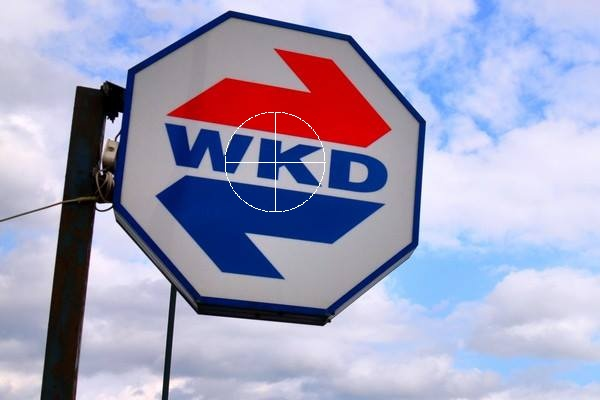
\includegraphics[width=\linewidth]{raw.jpg}
					\caption{Obraz wyjściowy}
				\end{subfigure}
				\begin{subfigure}[b]{0.45\linewidth}
					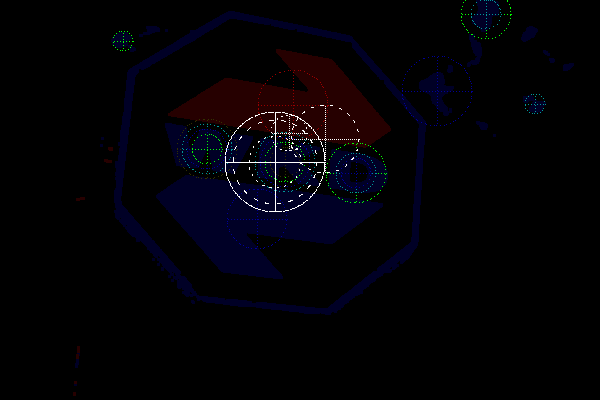
\includegraphics[width=\linewidth]{output.png}
					\caption{Znalezione obiekty}
				\end{subfigure}
		\end{figure}
		Na lewym obrazku jest wejściowy obraz z zaznaczonym znalezionym logiem.
		
		Na prawym obrazku są zaznaczone obiekty, wyznaczone w trakcie pracy.
		Małymi, przerywanymi okręgami zaznaczono wstępne dopasowania poszczególnych obiektów.
		Odcienie zielonego oznaczają kolejne litery.
		
		Większymi okręgami zaznaczono obiekty znalezione po szukaniu konfiguracji, porównując odległości obiektów.
		Jak widać w tym przypadku pierwsze dopasowanie było od razu najlepsze.
		
		Białym krzyżem zaznaczono środek, czyli punkt między czerwoną, a niebieską strzałką.
		
	\section{Możliwości rozwoju}
		Ponieważ program jest napisany obiektowo, z dużą ilością abstrakcji, możliwa jest implementacja innego algorytmu w oparciu o istniejące klasy.
		
		Można zrównoleglić poszukiwanie obiektów do dwóch wątków, co na wielordzeniowym komputerze przyspieszy działanie.
		Takich mniejszych akcji, jak sortowanie, nie trzeba przyspieszać, gdyż i tak dzieją się wystarczająco szybko, w porównaniu z innymi obliczeniami.
		
		Wykrywanie kilku logów na raz jest możliwe do dodania. Wystarczy, że na etapie szukania konfiguracji, program będzie potrafił zaakceptować kilka znalezisk.
		Do tego jest wymagane pogłębienie szukania wśród obiektów, co znacznie zwiększy ilość obliczeń.
		
		Aby ulepszyć jakość wykrywania, warto by użyć jakiegoś zaawansowanego systemu do obliczania parametrów programu.
		
\end{document}
